\subsubsection{Minuta de reunião (08-Julho-2015)}

\begin{tabbing}
  Local \= xxx \kill
  Local \> : LEAD \\
  Data  \> : 08 de Julho de 2015 \\
  Hora  \> : 13:00
\end{tabbing}

%---------------------------------------------------------------------
\participantes{
  \elael,
  \alana,
  \gabriel,
  \julia,
  \ramon,
  \renan.
}

\textbf{Aprovação da minuta}

\textbf{Update semanal do Projeto EMMA}

  
\textbf{\renan.} 
	\begin{itemize}
		\item \textbf{Tarefas concluídas:}
			\begin{itemize}    
				\item Pesquisa de braços robóticos com boa relaçào entre peso e alcance.
				KUKA KR10 com 6 graus de liberdade e 10kg de payload.
				\item Apresentação para Rijeza em Porto Alegre.
			\end{itemize}
		
		\item \textbf{Novas tarefas:}
			\begin{itemize} 
				\item Metodologia de análise para braços robóticos.
			\end{itemize}
	\end{itemize}
		
\textbf{\elael.} 
	\begin{itemize}
		\item \textbf{Tarefas concluídas:}
			\begin{itemize}    
				\item Estado da Arte para calibração de braços robóticos.
				\item Encontrou uma solução para reparo que menciona localização por 3D. 
			\end{itemize}
		
		\item \textbf{Novas tarefas:}
			\begin{itemize} 
				\item Encontrar uma forma de reduzir o peso dos cabos.(email Darlan)
			\end{itemize}
	\end{itemize}
					
			
   \textbf{\gabriel.} 
	\begin{itemize}
		\item \textbf{Tarefas concluídas:}
			\begin{itemize}    
				\item Estudo sobre sensores e seus respectivos drivers, pontos fracos e
				fortes, como se enquadrariam em nossa solução.  
			\end{itemize}
		
		\item \textbf{Novas tarefas:}
			\begin{itemize} 
			    \item Pesquisar Sensores 1D
			    \item Auxiliar workspace analisys de Rena e Estevão com Open Rave. 
			\end{itemize}
	\end{itemize}

			
\textbf{\estevão.} 
	\begin{itemize}
		\item \textbf{Tarefas concluídas:}
			\begin{itemize}    
				\item Pesquisa de braços robóticos com boa relaçào entre peso e alcance.
				KUKA KR10 com 6 graus de liberdade e 10kg de payload.
				\item Trabalhou com a hipótese de 4 posições para cobrir a pá.
			\end{itemize}
		
		\item \textbf{Novas tarefas:}
			\begin{itemize} 
				\item Metodologia de análise para braços robóticos.
				\item Estudar qual o alcance e graus de liberdade pra cobrir a pá.
			\end{itemize}
	\end{itemize}
	
		
   \textbf{\julia.} 
	\begin{itemize}
		\item \textbf{Tarefas concluídas:}
			\begin{itemize}    
				\item Estudo das tarefas do robô e seu mapeamento para a construção da
			    interface de usuário.
			    \item Apresentou organograma das tarefas do Robô com descrição de
				atividades da interface do usuário.
			\end{itemize}
		
		\item \textbf{Novas tarefas:}
			\begin{itemize} 
			 \item Fluxograma, pesquisar para descrever em fluxograma completo os
			 processos relacionados a calibração, Reparo, Metalização e Jatemaneto
			 \item Distinguir e detalhar cada processo de tarefas. 
			\end{itemize}
	\end{itemize}

			



\textbf{Agenda para a próxima reunião:}
  \begin{itemize}
    \item Resultado de pesquisas individuais.
    \item Novas tarefas \& recomendações.
  \end{itemize}


\vspace{5mm}%
\parbox[t]{70mm}{
  Aprovado por: \\[5mm]
  \centering
  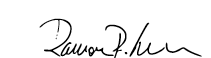
\includegraphics[width=65mm]{figs/logo/assinatura-ramon.png} \\[-4mm]
  \rule[2mm]{70mm}{0.1mm} \\
  \ramon \\[1mm]
  Coordenador do Projeto \\
}

%---------------------------------------------------------------------
\fim